\chapter{Preliminaries}

\label{chapter:preliminaries}
\section{Homogenous coordinate systems}

Homogenous coordinates are a tool to simplify certain geometrical operations by adding an extra dimension.
For example, the general scaling, rotation and translation are expressed in non-homogenous coordinates as:
% To transform a point $m=(u, v)^\top$ from cartesian coordinates to homogenous, simply append $1$ as the third coordinate: $m=(u, v, 1)^\top$.

\begin{equation}
    \vec{m}_1 = 
    \mat{S} \mat{R}
    \vec{m}_0
    + \vec{t},
\end{equation}

\begin{equation}
    \mat{S} = \begin{bmatrix} s_x & 0 \\ 0 & s_y \end{bmatrix}, \;\; 
    \mat{R} = \begin{bmatrix} \cos(\theta) & -\sin(\theta) \\ \sin(\theta) & \cos(\theta) \end{bmatrix}, \;\;
    \vec{t} = \begin{bmatrix} t_x \\ t_y \end{bmatrix},
\end{equation}

where $m_0$ is the original point,
$m_1$ is the transformed point, 
$\mat{S}$ is a scaling matrix,
$\mat{R}$ is a rotation matrix and 
$\vec{t}$ is a translation vector.

The same operations can be expressed in a homogenous coordinate system using only matrix multiplication as

\begin{equation}
    \begin{bmatrix} \vec{m}_1 \\ 1 \end{bmatrix} = 
    \begin{bmatrix}
        \mat{S} \mat{R} & \vec{t} \\
        \vec{0}^\top & 1
    \end{bmatrix}
    \begin{bmatrix} \vec{m}_0 \\ 1 \end{bmatrix} = 
    \mat{S}_H \mat{R}_H \mat{T}_H
    \begin{bmatrix} \vec{m}_0 \\ 1 \end{bmatrix},
\end{equation}
\begin{equation}
    \mat{S}_H = \begin{bmatrix} s_x & 0 & 1\\ 0 & s_y & 1 \\ 0 & 0 & 1\end{bmatrix}, \;\;
    \mat{R}_H = \begin{bmatrix} \cos(\theta) & -\sin(\theta) & 0 \\ \sin(\theta) & \cos(\theta) & 0 \\ 0 & 0 & 1 \end{bmatrix}, \;\;
    \mat{T}_H = \begin{bmatrix} 1 & 0 & t_x\\ 0 & 1 & t_y \\ 0 & 0 & 1 \end{bmatrix} ,
\end{equation}
where $\mat{S}_H, \mat{R}_H$ and $\mat{T}_H$ are homogenous transformation matrices.

So in the homogenous coordinate system, these transformations can be combined and expressed as matrix multiplications.

\section{Pinhole camera model}
\label{sec:pinhole_camera_model}
A pinhole camera, the canonical perspective camera model - is a model of a simple camera without any optics.
The first example is the camera obscura - a dark room with a small hole through which the image from outside is projected on the opposite wall. 
This model can be used to express camera geometry with a field of view angles less than $180^{\circ}$.

\subsection{Camera coordinate system}
\begin{figure}[ht]
    \centering
    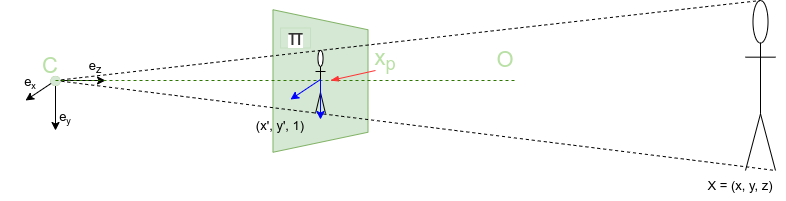
\includegraphics[width=\textwidth]{graphics/td_scene.png}
    \caption{The scheme of a pinhole camera model.}
    \label{fig:td_scene_3d}
\end{figure}

\begin{figure}[ht]
    \centering
    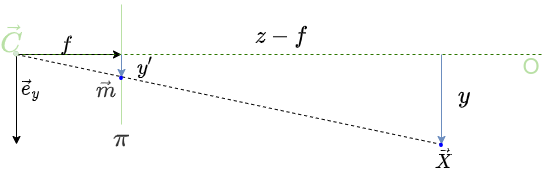
\includegraphics[width=\textwidth]{graphics/td_scene_yz.png}
    \caption{The pinhole camera model, y-z plane.}
    \label{fig:td_scene_yz}
\end{figure}

\begin{figure}[ht]
  \centering
  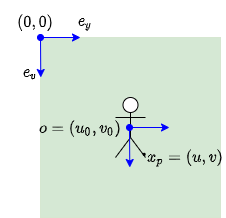
\includegraphics[width=0.4\textwidth]{graphics/td_scene_xy.png}
  \caption[The pinhole camera model, x-y plane.]{The pinhole camera model, x-y plane.}
  \label{fig:td_scene_xy}
\end{figure}

\begin{figure}[ht]
  \centering
  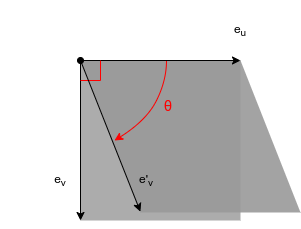
\includegraphics[width=0.49\textwidth]{graphics/pixel.png}
  \caption[A scheme of a skewed pixel.]{A scheme of a skewed pixel. $\vec{e}_u$ and $\vec{e}_v$ are the image basis vectors, where $\lVert \vec{e}_u \rVert = \frac{w_s}{w_{im}}$, $\lVert \vec{e}_v \rVert = \frac{h_s}{h_{im}}$, $w_s$ and $h_s$ are physical width and height of a camera sensor, $w_{im}$ and $h_{im}$ are the image width and height in pixels. $\vec{e}_v'$ is an edge of the skewed pixel and $\theta$ is the skew angle.}
  \label{fig:Kframes}
\end{figure}

In the physical implementation of the camera obscura, the projective plane is on the opposite side from the projection center (or camera center $\vec{C}$ in the pinhole camera model), and the image is reversed and mirrored. 
However, in most computer vision literature, authors assume that it is on the same side as the object (see \autoref{fig:td_scene_3d}).
In \autoref{fig:td_scene_3d} a camera with camera center $\vec{C}$ in a coordinate system with origin at $\vec{C}$ and basis vectors $(\vec{e}_x, \vec{e}_y, \vec{e}_z)$ is observing a human. 
Each point $\vec{X} = (x, y, z)^\top$ in a world coordinate system has a projection $\vec{m} = (u, v)^\top$ on a plane $\pi$ which is located at distance $f$ from the camera center (refer to \autoref{fig:td_scene_yz}). 
The optical axis $\vec{O}$ is a ray perpendicular to plane $\pi$, and on the image the point $ \vec{O} \cap \pi = \vec{o}$ is the center of the image, see \autoref{fig:td_scene_xy}.

\subsection{Camera matrix}
The camera calibration matrix is a matrix that includes the camera's \textit{intrinsic} parameters - focal length, pixel skew angle $\theta$ (illustrated in \autoref{fig:Kframes}) and principle point coordinates $\vec{o} = (u_0, v_0)$ (see \autoref{fig:td_scene_xy}).
The camera calibration matrix can be expressed as
\begin{equation}
    \mat{K} = \begin{bmatrix}
        f_x & -f_x \cot(\theta) & u_0 \\
        0 & f_y & v_0 \\
        0 & 0 & 1 \\
    \end{bmatrix},
    \textrm{\;units: } [f_x]=\textrm{px},\; [f_y]=\textrm{px},\; [u_0]=\textrm{px},\; [v_0]=\textrm{px},
\end{equation}

where $f_x = \frac{f}{\lVert \vec{e}_u \rVert} $ and $f_y = \frac{f}{\lVert \vec{e}_v \rVert \sin{\theta}}$ represents the focal length of a camera in the horizontal and vertical image units.
$\vec{e}_u$ and $\vec{e}_v$ are the image basis vectors (refer to \autoref{fig:Kframes}) and $f$ is a focal length, $[f] = m$ .

Most modern digital cameras have no skew and square pixels, so in most cases, the camera matrix can be simplified to:

\begin{equation}
    \label{eq:kmat}
    \mat{K} = \begin{bmatrix}
        f_x & 0 & u_0 \\
        0 & f_y & v_0 \\
        0 & 0 & 1 \\
    \end{bmatrix}.
\end{equation}

\subsection{Projection matrix}

\begin{figure}[ht]
    \centering
    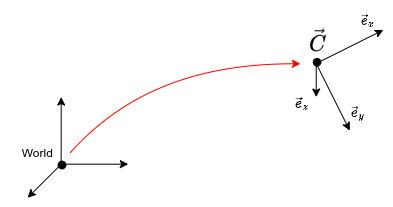
\includegraphics[width=.5\textwidth]{graphics/frames.png}
    \caption{Transformation from world to camera coordinate frames.}
    \label{fig:frames}
\end{figure}

To translate a point from a world coordinate frame to an image coordinate frame, the image projection matrix $\mat{P}$ is used. 
The canonical projection matrix $\mat{P}_0$ assumes that the camera is in the world coordinate center and that the calibration matrix $\mat{K} = \mat{I}$.
$\mat{P}_0$ is expressed as
\begin{equation}
\mat{P}_0 = \begin{bmatrix} \mat{I} & | & \vec{0} \end{bmatrix} = 
    \begin{bmatrix}
    1 & 0 & 0 & 0 \\
    0 & 1 & 0 & 0 \\
    0 & 0 & 1 & 0 \\
    \end{bmatrix}.
\end{equation}

However, this case is impractical. 
The canonical projection matrix is not used in practice because each real camera is different. 
Instead, the image projection matrix $\mat{P}$ is used with a camera matrix $\mat{K}$ to transform the canonical $\mat{P}_0$ to the specific $\mat{P}$:

\begin{equation}
\mat{P} = \mat{K} \begin{bmatrix} \mat{I} & | & \vec{0} \end{bmatrix} = 
    \begin{bmatrix} 
    f_x & 0 & u_0 & 0 \\
    0 & f_y & v_0 & 0 \\ 
    0 & 0 & 1 & 0 \\
    \end{bmatrix}.
\end{equation}

The world coordinate center is usually not located at point $\vec{C}$ as ilustrated in \autoref{fig:frames}. 
It may be rotated using a rotation matrix $\mat{R}$ and translated by a vector $\vec{t}$ where $\mat{R}$ is a $3x3$ matrix with $\det(\mat{R}) = 1$ and $\mat{R}^{-1} = \mat{R}^\top$. 
Therefore, in the general case the projection can be expressed as
\begin{equation}
    \label{eq:PKRt}
    \mat{P} = \mat{K} \begin{bmatrix} \mat{R} & | & \vec{t} \end{bmatrix} = 
    \mat{K} \begin{bmatrix} \mat{R} & | & - \mat{R} \vec{C} \end{bmatrix},
\end{equation}
where $\vec{C}$ is the camera's position in the world reference frame. 

Image point $\vec{m} = (u, v)^\top$ can be obtained from a 3D point $\vec{X}$ using the projection matrix $\mat{P}$ as

\begin{equation}
    \label{eq:projection}
    \lambda \begin{bmatrix} 
        u \\ v \\ 1 \end{bmatrix} = \mat{P} \begin{bmatrix} x \\ y \\ z \\ 1
    \end{bmatrix},
\end{equation}

\begin{equation}
    \label{eq:proj_min}
    \lambda 
    \begin{bmatrix} 
    \vec{m} \\ 1 \end{bmatrix} = \mat{P} \begin{bmatrix} \vec{X} \\ 1
    \end{bmatrix},
\end{equation}
where $\lambda > 0$ is a free scaling parameter.

\subsection{Skew-symmetric 3x3 matrix}
A skew-symmetric or antisymetric matrix of vector $\vec{b} = (b_1, b_2, b_3)^\top$ is defined as
\begin{equation}
    [\vec{b}]_{\times} = \begin{bmatrix}
        0 & -b_3 & b_2 \\ 
        b_3 & 0 & -b_1 \\ 
        -b_2 & b_1 & 0 \\ 
    \end{bmatrix}.
\end{equation}

This matrix has several useful properties, but the most important in this thesis is that it generalizes a cross product as matrix multiplication:
\begin{equation}
    \vec{a} \times \vec{b} = [\vec{a}]_{\times} \vec{b}.
\end{equation}
The notation is taken from \cite{hartley_zisserman_2004}, p. 581.

\section{Epipolar geometry}

\label{sec:epipolar_geometry}
\begin{figure}[ht]
    \centering
    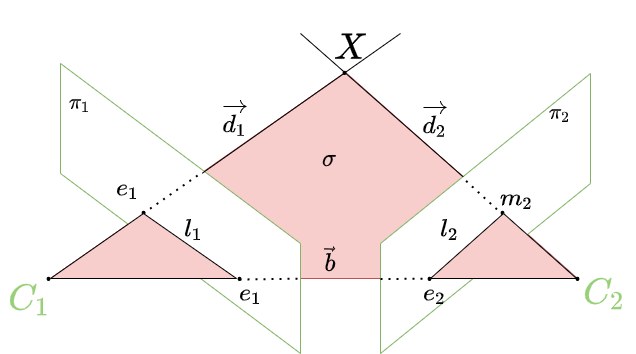
\includegraphics[width=\textwidth]{graphics/epipolar.png}
    \caption{A scheme of epipolar geometry.}
    \label{fig:epipolar_std}
\end{figure}

\autoref{fig:epipolar_std} shows a scheme of two cameras with different optical centers $\vec{C}_1$ and $\vec{C}_2$ connected with a base vector $\vec{b} = \vec{C}_2 - \vec{C}_1$. 
Both of the cameras observe the same 3D point $\vec{X}$. 
Projections of this point to $\pi_1$ and $\pi_2$ are $\vec{m}_1$ and $\vec{m}_2$, respectively. 
Points $\vec{C}_1$, $\vec{C}_2$ and $\vec{X}$ form an \textit{epipolar plane} $\sigma$.
The lines $\sigma \cap \pi_1 = l_1$ and $\sigma \cap \pi_2 = l_2$ are \textit{epipolar lines}. 
The epipolar line $l_1$ passes through an \textit{epipole} $\vec{e}_1$ and through point $\vec{m_1}$, where $\lambda [\vec{e}_1 | 1]^\top = \mat{P}_1 \vec{C}_2$.
Similarly, line $l_2$ passes through an \textit{epipole} $\vec{e}_2$ and through point $\vec{m_2}$, where $\lambda [\vec{e}_2 | 1]^\top = \mat{P}_2 \vec{C}_1$.

\subsection{The epipolar constraint}
Having a set of two cameras, the relationship between them and the constraints on them can be expressed by two matrices: the \textit{essential matrix} $\mat{E} \in \mathbb{R}^{3x3}$, $(\rank(\mat{E}) = 2)$, and the \textit{fundamental matrix} $\mat{F} \in \mathbb{R}^{3x3}$, $(\rank(\mat{F}) = 2)$. Matrix $\mat{E}$ is obtained as
\begin{equation}
    \label{eq:E}
    \mat{E} = \mat{R}_2 [\vec{C}_2 - \vec{C}_1]_{\times} \mat{R}_1^\top = [-\vec{t}_{21}]_{\times} \mat{R}_{21} = [\vec{b}]_{\times} \mat{R}_{21},
\end{equation}
and matrix $\mat{F}$ as
\begin{equation}
    \label{eq:F}
    \mat{F} = \mat{K}_2^{-T} \mat{R}_2 [\vec{C}_2 - \vec{C}_1]_{\times} \mat{R}_1^\top \mat{K}_1^{-1} = 
    \mat{K}_2^{-T} [-\vec{t}_{21}]_{\times} \mat{R}_{21} \mat{K}_1^{-1} = 
    \mat{K}_2^{-T} \mat{E} \mat{K}_1^{-1},
\end{equation}
where 
$\mat{R}_i$ and $\vec{t}_i$ are rotation and translation of the $i$-th camera in the worls coordinate frame, $i \in \{1, 2\}$,
$\mat{R}_{21} = \mat{R}_2 \mat{R}_1^\top$ is a relative camera rotation and 
$\vec{t}_{21} = -\mat{R}_2 \vec{b} = \vec{t}_2 - \mat{R}_{21}\vec{t}_1$ is a relative camera translation.

An algebraic expression of the important properties of matrix $\mat{F}$ using notation from \autoref{sec:epipolar_geometry} are:
\begin{equation}
    \label{eq:Fm2}
    l_1 = \mat{F}^\top \begin{bmatrix} \vec{m}_2 \\ 1 \end{bmatrix},
\end{equation}
\begin{equation}
    \label{eq:Fm1}
    l_2 = \mat{F} \begin{bmatrix} \vec{m}_1 \\ 1 \end{bmatrix},
\end{equation}
\begin{equation}
    \label{eq:fefe}
    \mat{F} \begin{bmatrix} \vec{e}_1 \\ 1 \end{bmatrix} = \mat{F}^\top \begin{bmatrix} \vec{e}_2 \\ 1 \end{bmatrix} = 0,
\end{equation}
\begin{equation}
    \label{eq:epiconstr}
    \begin{bmatrix} \vec{m}_2 & | & 1 \end{bmatrix} \mat{F} \begin{bmatrix} \vec{m}_1 \\ 1 \end{bmatrix} = 0.
\end{equation}
Matrix $\mat{F}$ maps points from $\pi_1$ to epipolar lines on $\pi_2$ and vice versa (eqs. \eqref{eq:Fm2} and \eqref{eq:Fm1}); epipoles $\vec{e}_1$ and $\vec{e}_2$ are basis vectors of the right and left nullspaces of $\mat{F}$, respectivly (eq. \eqref{eq:fefe}).
Epipolar constraint described by eq. \eqref{eq:epiconstr} means that a point and its correspondent line are on the same plane (see \autoref{fig:epipolar_std}).

\section{Stereo vision}

\begin{figure}[ht]
    \centering
    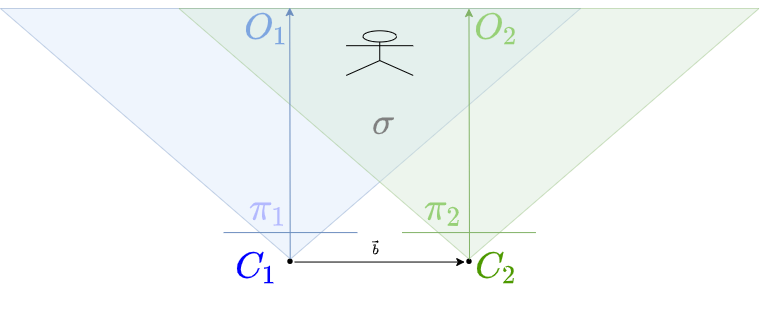
\includegraphics[width=0.8\textwidth]{graphics/stereopair.png}
    \caption[Illustration of a typical stereocamera setup.]{Illustration of a typical stereocamera setup. Two cameras have optical centers at $\vec{C}_1$ and $\vec{C}_2$ and projection planes $\pi_1$ and $\pi_2$.
    The base vector between the camera centers is shown as a vector $\vec{b} = \vec{C}_2 - \vec{C}_1$. 
    Both cameras have parallel optical axes $\vec{O}_1$ and $\vec{O}_2$. 
    The common area visible by both cameras is marked as $\Psi$.}
    \label{fig:sch_stereo}
\end{figure}
\begin{figure}[ht]
    \centering
    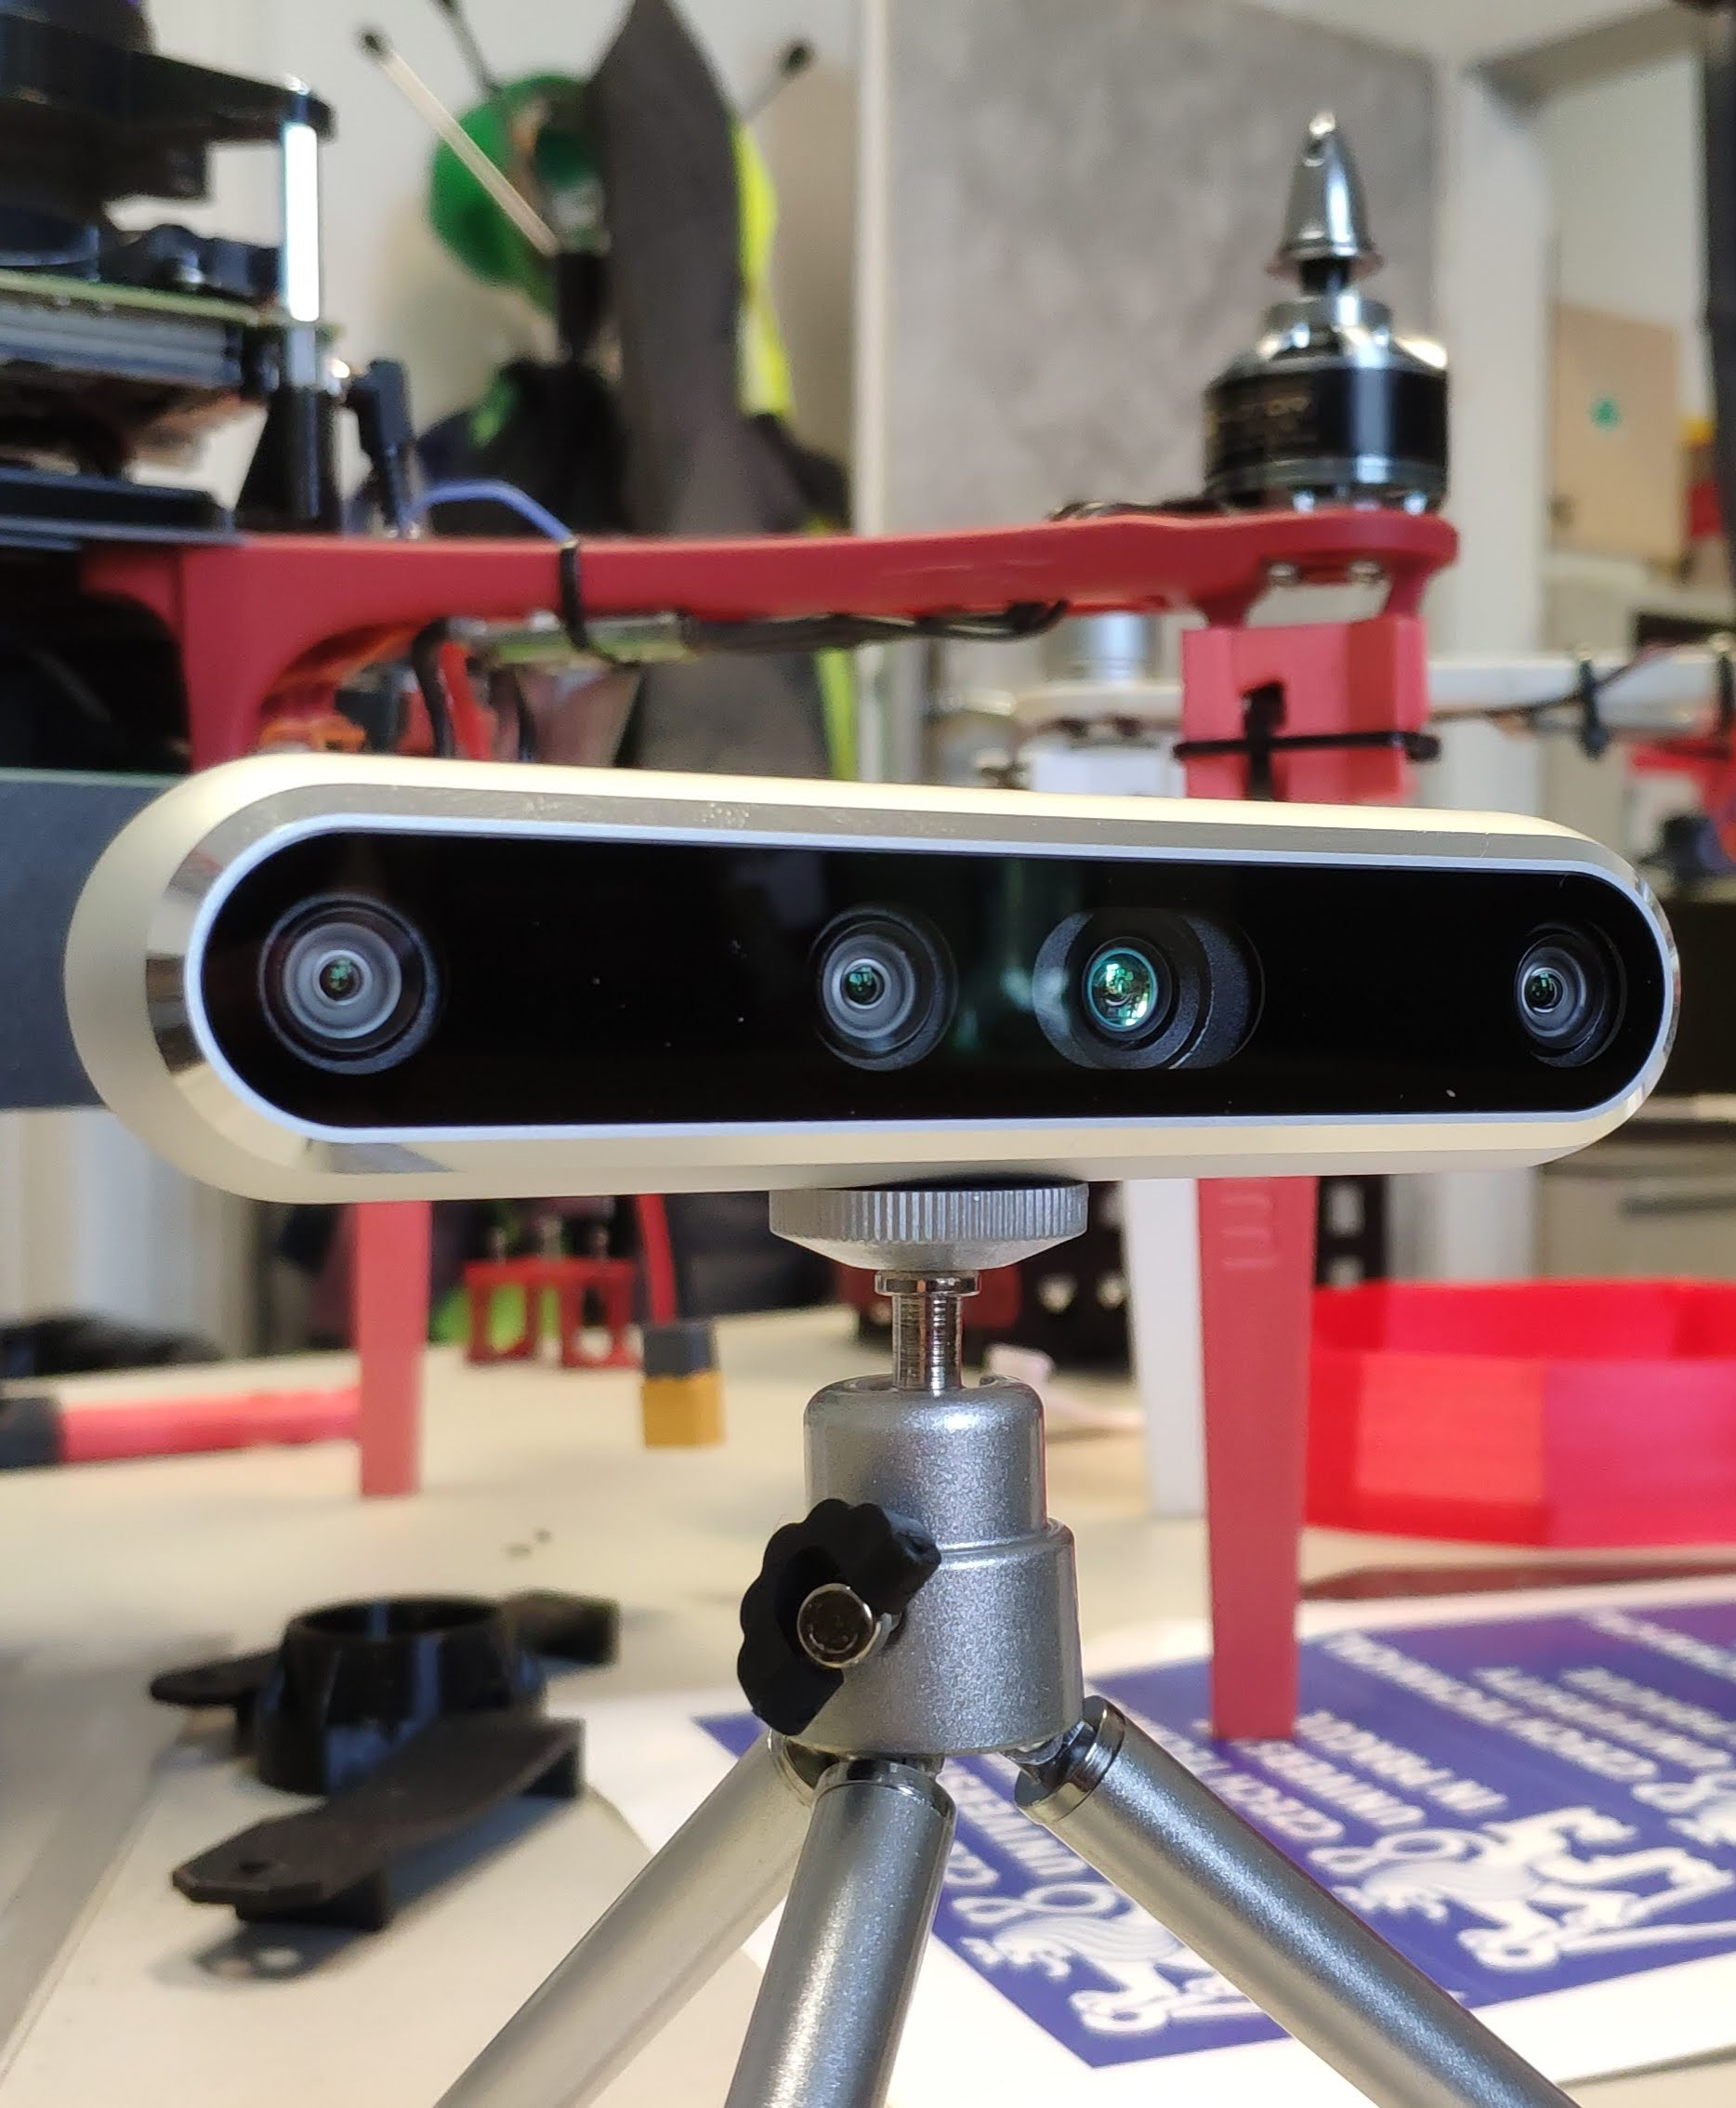
\includegraphics[width=0.3\textwidth]{graphics/stereo_example.jpg}
    \caption[An example of an industrial stereocamera.]{An example of an industrial stereocamera Intel Realsense D455.}
    \label{fig:inteld455}
\end{figure}

A typical digital image represents 2D information about a scene projected onto the image plane as in \autoref{fig:td_scene_3d}.
Computer stereo vision is a process of extracting a depth image from a pair of images of the same scene. 
Such depth images are often used in SLAM, obstacle avoidance or detailed reconstruction of the environment in robotics.
In \autoref{chapter:intro}, the most common methods of stereo vision are described.
Among the scene depth estimation approaches there are the computationally expensive neural network-based monocular approaches and costly LiDAR sensors.
A typical stereo camera is a tradeoff between price and processing complexity.

Usually, a stereo camera has a pair of cameras located at a distance $\lVert \vec{b} \rVert$ pointing in the same direction, similarly to the human eye (a scheme is in \autoref{fig:sch_stereo}).
Sometimes, a fusion of multiple cameras and other sensors is used, such as in the case of the Intel Realsense shown in \autoref{fig:inteld455} that has two IR cameras, a color sensor and an infra red projector to project some features onto the environment in there are insufficient features already present (for example when observing a white wall).

\section{Reprojection error}
\label{sec:error_reprojection}
In an ideal case, when the calibration matrix $\mat{K}$ has no error and the estimated transformation between the two cameras of the stereopair is accurate, rays $\vec{d}_1$ and $\vec{d}_2$ corresponding to the 3D projections of $\vec{m}_1$ and $\vec{m}_2$ (refer to \autoref{fig:epipolar_std}) intersect in the point $\vec{X}$. 
However, calibration only estimates the parameters up to some precision because of noise, measurement errors, limited resolution of the cameras etc.
The reprojection error is used to measure this precision.

After the 3D position of a point is computed based on its projections to the two cameras, to measure its reprojection error, it is projected back to an image, and a distance of this reprojection from the original projection that was used to obtain the 3D positiom estimate is computed.
Consider a general projection matrix $\mat{P}_i$ as
\begin{equation}
    \label{eq:p_general}
    \mat{P}_i = \begin{bmatrix} 
        (\vec{p}_{i, 1})^\top \\ 
        (\vec{p}_{i, 2})^\top \\ 
        (\vec{p}_{i, 3})^\top \end{bmatrix}.
\end{equation}
The reprojection error is defined as 
\begin{equation}
    e^2(\underline{X}) = \sum_{c=1}^{2}{  
    \begin{bmatrix}
        \begin{pmatrix}
            u_c - \frac{(\vec{p}_{c, 1})^\top \underline{X}}{(\vec{p}_{c, 3})^\top \underline{X}}
        \end{pmatrix}^2 + 
        \begin{pmatrix}
            v_c - \frac{(\vec{p}_{c, 2})^\top \underline{X}}{(\vec{p}_{c, 3})^\top \underline{X}}
        \end{pmatrix}^2
    \end{bmatrix}
    },
\end{equation}
where $m_c = \begin{bmatrix} u_c \\ v_c \end{bmatrix}$, $\underline{X} = \begin{bmatrix} \vec{X} \\ 1 \end{bmatrix}$ and $c$ corresponds to the camera index.
